\section{LatentRisk-VLM}
\subsection{Problem Setup}
Let $f_I$ and $f_T$ be frozen image and text encoders. For image $x_i$ and class prompt $p_c$, the unit-normalized embeddings are $z_i=f_I(x_i)\in\mathbb{R}^d$ and $t_c=f_T(p_c)\in\mathbb{R}^d$. Frozen zero-shot prediction is
\begin{equation}
 \hat y_i^{\mathrm{zs}}=\arg\max_{c\in\mathcal{Y}} z_i^\top t_c.
\end{equation}

We observe a calibration set $D_{\mathrm{cal}}=\{(x_i,y_i)\}_{i=1}^n$ with task labels but no group attributes. A group attribute $a_i$ (place in Waterbirds or gender in CelebA) may be revealed only after model selection to compute group accuracy. The primary protocol forbids $a_i$ during direction discovery, intervention, hyperparameter selection, and test-time scoring.

The calibration margin and risk are
\begin{align}
 m_i &= z_i^\top t_{y_i}-\max_{c\ne y_i}z_i^\top t_c,\\
 \rho_i &= \sigma(-m_i/\tau), \qquad h_i=\mathbb{I}[\rho_i\geq\eta].
\end{align}
A negative margin is a zero-shot error, so with the measured setting $\eta=0.5$, $h_i$ separates errors from correct predictions, where $h_i=1$ indicates an incorrect zero-shot prediction and $h_i=0$ indicates a correct zero-shot prediction. We seek a class-conditional, low-rank representation $U_c$ with three properties: it predicts $h_i$ after class semantics are removed, has weak coupling to the class score, and can be suppressed without erasing the score needed for class $c$. These properties define a latent risk subspace; they do not imply that $U_c$ encodes a named sensitive attribute. 

%  i think 14 line can write more

At test time $y$ is unknown. ``Class-conditional'' therefore cannot mean selecting $U_y$ with the ground-truth label. For every candidate $c$, the method constructs a corrected embedding $\hat z^{(c)}$ and score $s_c(x)$, then predicts $\arg\max_c s_c(x)$. This candidate-wise rule is part of the problem definition and prevents test-label leakage.

% 18 line i think A bit hard to understand

Figure~\ref{fig:pipeline} shows the complete pipeline. The backbone is used only to encode images and text; all subsequent operations occur in its normalized embedding space.

\begin{figure*}[t]
\centering
% The original TikZ flowchart is retained here for reference:
% \begin{tikzpicture}[
%   node distance=4mm,
%   box/.style={draw, rounded corners=1.5pt, align=center, minimum height=9mm,
%               text width=2.20cm, font=\small},
%   flow/.style={-{Latex[length=2mm]}, line width=0.5pt}
% ]
% \node[box] (vlm) {Frozen image and text encoders};
% \node[box, right=of vlm] (risk) {Task-label margin\\risk $h_i$};
% \node[box, right=of risk] (resid) {Class-semantic\\residual $\tilde z_i$};
% \node[box, right=of resid] (direction) {Risk-direction\\estimator $U_c$};
% \node[box, right=of direction] (edit) {Candidate-wise\\edit $\hat z^{(c)}$};
% \node[box, right=of edit] (score) {Classification or\\retrieval scores};
% \draw[flow] (vlm) -- (risk);
% \draw[flow] (risk) -- (resid);
% \draw[flow] (resid) -- (direction);
% \draw[flow] (direction) -- (edit);
% \draw[flow] (edit) -- (score);
% \node[font=\footnotesize, below=3mm of resid, xshift=12mm] {Calibration uses task labels $y$, but no group attribute $a$; the VLM weights remain fixed.};
% \end{tikzpicture}

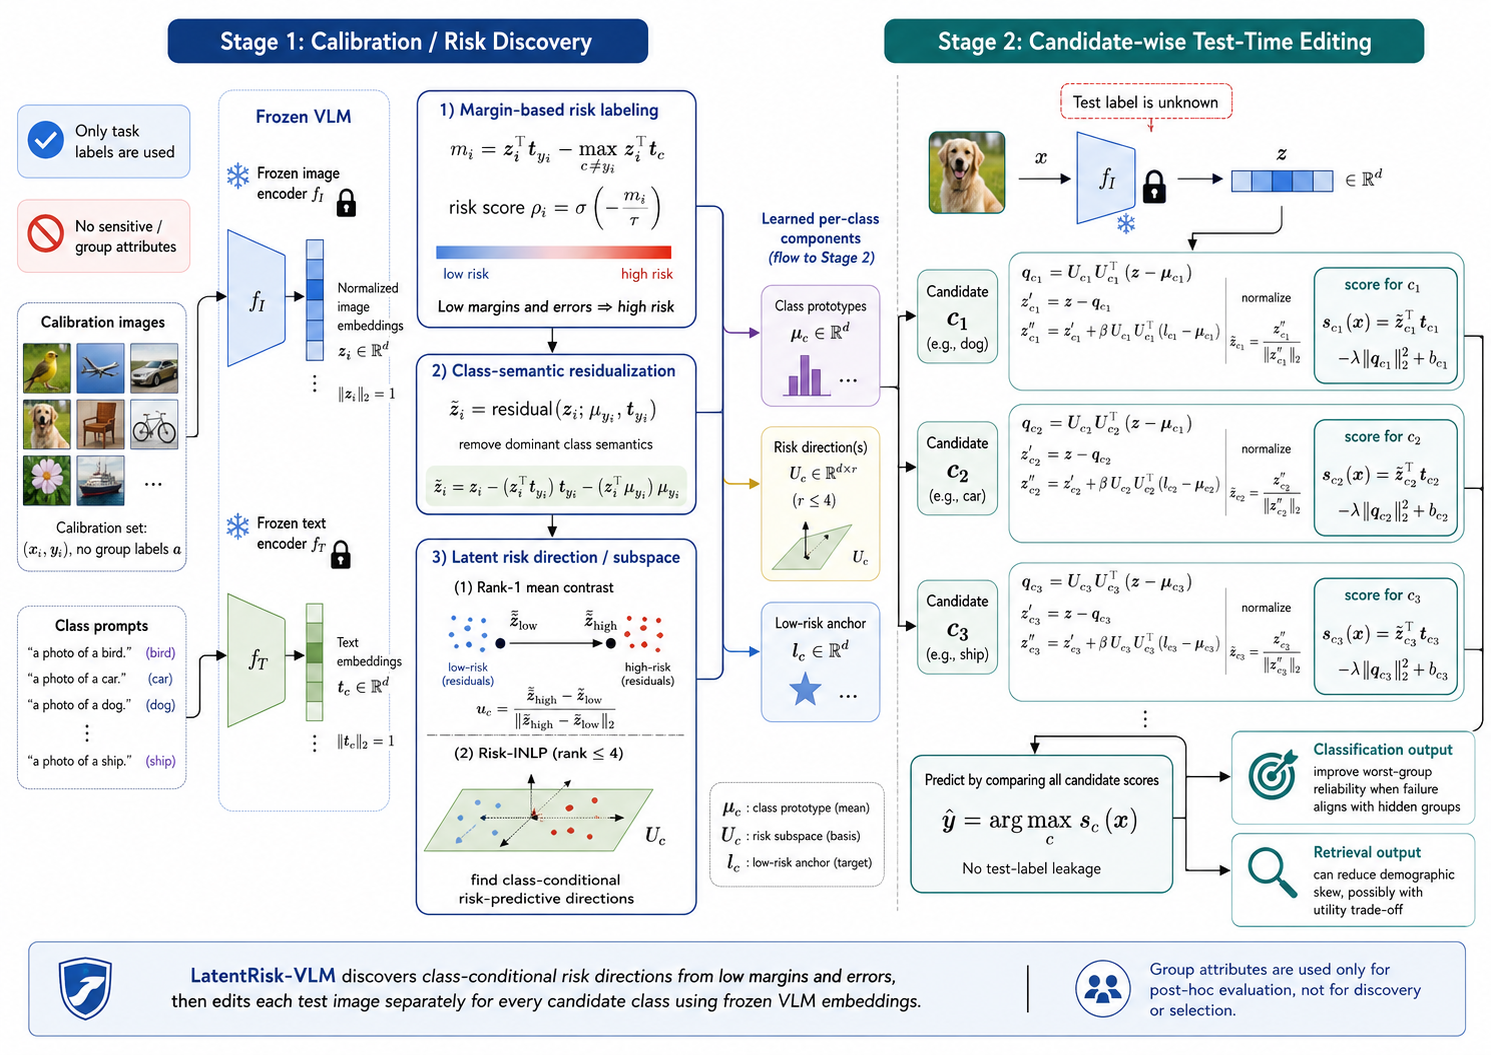
\includegraphics[width=\textwidth]{figures/picture.png}
\caption{\textsc{LatentRisk-VLM}. Risk directions are estimated from high- and low-risk residuals using mean contrast or iterative probes. At test time every candidate class is scored with its own correction; no test label selects the edit.}
\label{fig:pipeline}
\end{figure*}

\subsection{Removing Class-Level Semantics}
A risk estimator applied directly to $z_i$ may rely on ordinary
class-discriminative evidence rather than features genuinely associated
with classification error. For each class $c$, we therefore compute a
class prototype, defined as the mean embedding of its calibration samples:
\begin{equation}
 \mu_c=\frac{1}{|D_c|}\sum_{i:y_i=c}z_i,
\end{equation}
and form a residual orthogonal to the class text embedding:
\begin{equation}
 r_i=z_i-\mu_{y_i}, \qquad
 \tilde z_i=r_i-t_{y_i}t_{y_i}^{\top}r_i.
 \label{eq:residual}
\end{equation}
Subtracting the class prototype restricts risk-direction discovery to
within-class variation, while the second operation reduces the direct coupling between the representation and the corresponding class-prompt direction. However, these operations do not guarantee that all class information has been completely removed.

\paragraph{Unified design objective.}
We aim to identify a risk direction, or risk subspace, \(U_c\) that captures error-related information while containing as little class-semantic information as possible, such that suppressing it does not impair the classification capability. A compact specification is

% \begin{equation}
% \begin{aligned}
% \min_{U_c,\,\hat z^{(c)}}\quad
% &\mathcal{L}_{\mathrm{risk}}(U_c;\tilde Z_c,h_c) 
%  +\alpha\|t_c^{\top}U_c\|_2^2\\
% &\qquad +\lambda\|U_cU_c^{\top}(z-\mu_c)\|_2^2 -\hat z^{(c)\top}t_c\\
% \text{s.t.}\quad &U_c^{\top}U_c=I,\operatorname{rank}(U_c)\le r,\hat z^{(c)}=\operatorname{Edit}(z;U_c,\ell_c).
% \end{aligned}
% \label{eq:unified_objective}
% \end{equation}

\begin{equation}
\begin{aligned}
\min_{U_c,\,\hat z^{(c)}}\quad
&\mathcal{L}_{\mathrm{risk}}(U_c;\tilde Z_c,h_c)
+\alpha\|t_c^{\top}U_c\|_2^2\\
&\qquad+\lambda\|U_cU_c^{\top}(z-\mu_c)\|_2^2
-\hat z^{(c)\top}t_c .
\end{aligned}
\label{eq:unified_objective}
\end{equation}

Here, \(U_c^{\top}U_c=I\),\(\operatorname{rank}(U_c)\le r\), \(\hat z^{(c)}=\operatorname{Edit}(z;U_c,\ell_c)\).

% The first let found $U_C$ can predict risk. The second discourages class-semantic coupling. If this value is big, it means the risk direction is highly consistent with class text diretion, which means model learn class information rather than risk information. The third penalizes the candidate's risk activation. Project the features of the prototype samples of the removed category onto the risk subspace. If this value is large, it indicates that the sample contains a strong risk direction. Therefore, during the optimization process, we aim to reduce this activation. The fourth retains task semantics.Edited image embedding $\hat z^{(c)\top}$ still should maintain a high degree of similarity with the category text $t_c$. For constraint condition, \(U_c^{\top}U_c=I\) means the column vectors of $U_c$ are orthogonal.$U_c=[u_1,u_2,...,u_r]$ and $u_i^Tu_j=0$.\(\operatorname{rank}(U_c)\le r\) means only search for low-dimensional risk subspaces.\(\hat z^{(c)}=\operatorname{Edit}(z;U_c,\ell_c)\). Here $\operatorname{Edit}$ denotes the normalized candidate-wise projection and reinjection in Equations~\ref{eq:projection}--\ref{eq:score}, remove the risk direction through projection, and then inject neutral information. This is a design objective rather than an additional jointly optimized loss. In the implementation, class residualization reduces the semantic-coupling term, mean contrast or Risk-INLP estimates the risk term, projection implements suppressibility, and neutral reinjection plus the semantic score preserves utility. The scoring grid selects the operating point; $\alpha$ is not separately tuned.

The first term encourages the learned \(U_c\) to predict calibration risk. The second discourages coupling between the risk subspace and the class semantics. A large value of \(\|t_c^{\top}U_c\|_2^2\) indicates that the learned risk directions are strongly aligned with the class text embedding, suggesting that the model may be capturing class-discriminative information rather than risk-related information. The third term penalizes the candidate's activation in the risk subspace. Specifically, \(U_cU_c^{\top}(z-\mu_c)\) projects the class-centered feature onto the risk subspace. A large norm indicates that the candidate contains a strong risk component; therefore, the objective encourages this activation to be reduced. The fourth term preserves task semantics by encouraging the edited image embedding \(\hat z^{(c)}\) to remain highly similar to the class text embedding \(t_c\).

Regarding the constraints, \(U_c^{\top}U_c=I\) requires the columns of \(U_c\) to be orthonormal. In other words, for \(U_c=[u_1,u_2,\ldots,u_r]\), we have \(u_i^{\top}u_j=0\) for \(i\neq j\) and \(u_i^{\top}u_i=1\). The constraint \(\operatorname{rank}(U_c)\le r\) restricts the search to a low-dimensional risk subspace. Finally, \(\hat z^{(c)}=\operatorname{Edit}(z;U_c,\ell_c)\), where \(\operatorname{Edit}\) denotes the normalized candidate-wise projection and reinjection defined in Equations~\ref{eq:projection}--\ref{eq:score}: the risk component is first removed by projection, after which neutral information is reinjected.

This formulation is a design objective rather than an additional jointly optimized loss. In practice, class residualization reduces semantic coupling, mean contrast or Risk-INLP estimates the risk subspace, projection implements suppressibility, and neutral reinjection together with the semantic score preserves utility. The scoring grid determines the operating point, and \(\alpha\) is not tuned separately.

%  i think this can explain more clearly

\subsection{Estimating Risk Directions}
Let $H_c=\{i:y_i=c,h_i=1\}$ denote the set of high-risk or misclassified samples from class $c$, and let $L_c=\{i:y_i=c,h_i=0\}$ denote the corresponding low-risk or correctly classified samples. We estimate a class-specific risk direction by contrasting the mean residualized embeddings of these two groups:
\begin{equation}
 u_c=\frac{\bar z_{H_c}-\bar z_{L_c}}
 {\|\bar z_{H_c}-\bar z_{L_c}\|_2},
 \quad
 \bar z_S=\frac{1}{|S|}\sum_{i\in S}\tilde z_i.
 \label{eq:contrast}
\end{equation}
Here, $\bar z_{H_c}$ and $\bar z_{L_c}$ are the centroids of the high-risk and low-risk samples, respectively, in the residualized feature space. Their difference therefore points from the average representation of successful predictions toward that of failures. Normalizing this difference removes its scale and yields a unit vector that captures only the dominant direction of risk-related variation within class $c$.

Thus, $U_c=u_c\in\mathbb{R}^{d\times1}$ defines a one-dimensional, class-conditional risk subspace. For a residualized embedding $\tilde z_i$, the projection $u_c^\top \tilde z_i$ measures its activation along this direction, with larger values indicating greater alignment with the feature pattern associated with failures. The mean-contrast estimator provides the simplest linear description of how failures differ from successes after class residualization. Since it is constructed directly from the separation between high-risk and low-risk samples, it is risk-predictive by design. However, because no demographic or sensitive-attribute annotations are used, the resulting direction should be interpreted only as a latent risk direction rather than as a named demographic direction.

\paragraph{Probe-based directions.}
Alternatively, we fit a linear logistic probe to $h_i$ within each class. Its normalized weight becomes $u_{c,1}$; the residuals are projected into its null space, and the process repeats up to rank four or until probe accuracy falls below 0.55. QR orthogonalization yields $U_c=[u_{c,1},\ldots,u_{c,r}]$. This Risk-INLP estimator follows the iterative removal principle of \citet{ravfogel2020inlp}. Rank one tests a single discriminative direction, while rank four tests whether residual risk remains distributed after successive projections.

\subsection{Candidate-Wise Representation Editing}
For a test embedding $z$ and candidate class $c$, define its residual risk component $q_c=U_cU_c^\top(z-\mu_c)$. Full projection gives
\begin{equation}
 z'^{(c)}=z-q_c.
\label{eq:projection}
\end{equation}
Projection may move an embedding away from regions represented by low-risk calibration examples. Let $\ell_c$ be the mean original embedding over $L_c$. We reinsert half of its risk-subspace component,
\begin{equation}
 z''^{(c)}=z'^{(c)}+\beta U_cU_c^\top(\ell_c-\mu_c),
 \qquad \beta=0.5,
 \end{equation}
and normalize $\hat z^{(c)}=z''^{(c)}/\|z''^{(c)}\|_2$. The candidate score is
\begin{equation}
 s_c(x)=\hat z^{(c)\top}t_c-\lambda\|q_c\|_2^2+b_c.
 \label{eq:score}
\end{equation}
The first term retains CLIP semantic matching, the second penalizes candidate-specific risk activation, and $b_c$ is a class intercept. Prediction compares Equation~\ref{eq:score} over all $c$; it never applies a correction chosen by the ground-truth test class.

\subsection{Task-Label-Only Selection}
We choose $\lambda$ and $b_c$ on calibration data using accuracy (CelebA) or macro class accuracy (Waterbirds), with overall accuracy and smaller intervention parameters as tie breakers. Subspace rank, projection strength, and $\beta$ are fixed before this grid search. The primary selection score depends on $y$ but not $a$. For diagnosis, we rerun the same search using validation WGA over $(y,a)$ and label the resulting row \emph{attribute oracle}. Comparing the two selectors isolates a practical question: even if error-derived directions contain group-relevant information, can an attribute-free criterion choose a useful operating point?

\paragraph{Complexity.}
Using cached embeddings of dimension $d$, rank-1 discovery requires one pass over $n$ calibration samples, $O(nd)$ time and $O(nd)$ storage. Candidate-wise inference costs $O(|\mathcal{Y}|d)$ per image beyond the encoder call. The rank-$r$ extension increases projection cost to $O(|\mathcal{Y}|dr)$ and fits at most $r$ linear probes per class. No variant adds a VLM forward pass or modifies backbone parameters.

\subsection{Retrieval Adaptation}
For Flickr30K calibration captions, risk is the negative margin between the paired image and the hardest nonmatching image. Paired image embeddings are centered by their global prototype and residualized against their caption embeddings. Splitting at the median margin yields one high--low risk direction. The same projection and reinjection edit every gallery image, while $\lambda$ is selected by validation text-to-image Recall@10. The fitted editor is then evaluated unchanged on Flickr30K test retrieval and on FairFace demographic skew; FairFace gender labels never enter fitting or ranking.
